\documentclass{article}
\usepackage{ctex}
\usepackage{amsmath}
\usepackage{amssymb}
\usepackage{graphicx}
\usepackage{float}
\usepackage{multirow}
\usepackage{verbatim}
\usepackage{subfigure}
\usepackage{color}
\usepackage{enumerate}
\usepackage{enumitem}
\usepackage{geometry}
\usepackage{listings}
\usepackage{fontspec}
\newfontfamily\jetbrains{JetBrains Mono}
\lstset{
    breaklines,                                 % 自动将长的代码行换行排版
    extendedchars=false,                        % 解决代码跨页时,章节标题,页眉等汉字不显示的问题
    backgroundcolor=\color[rgb]{0.96,0.96,0.96},% 背景颜色
    keywordstyle=\color{blue}\bfseries,         % 关键字颜色
    identifierstyle=\color{black},              % 普通标识符颜色
    commentstyle=\color[rgb]{0,0.6,0},          % 注释颜色
    stringstyle=\color[rgb]{0.58,0,0.82},       % 字符串颜色
    showstringspaces=false,                     % 不显示字符串内的空格
    numbers=left,                               % 显示行号
    numberstyle=\tiny\jetbrains,                    % 设置数字字体
    basicstyle=\small\jetbrains,                    % 设置基本字体
    captionpos=t,                               % title在上方(在bottom即为b)
    frame=single,                               % 设置代码框形式
    rulecolor=\color[rgb]{0.8,0.8,0.8},         % 设置代码框颜色
}
\usepackage{hyperref}
\hypersetup{
    hypertex=true,
    colorlinks=true,
    linkcolor=black,
    anchorcolor=black,
    citecolor=black,
}

\title{区块链实验四 实验报告}
\author{PB19071405 王昊元}
\date{2022 年 06 月 25 日}

\begin{document}
    \maketitle
    \section{实验目的及要求}
    \subsection{实验目的}
    \begin{itemize}
        \item 了解fabric上的链码部署和配置
        \item 开发fabric上的链码
        \item 实现一个fabric上的链码和功能
    \end{itemize}
    \subsection{实验目标档次及要求}
    \begin{itemize}
        \item 目标档次:B
        \item 要求:实现一个能够体现增删改查功能的链码,参考官方的例子即可,应用的业务场景不是考察的重点。部署并正确调用链码,截图。提交源码和实验报告。
    \end{itemize}
    \section{实验平台}
    \begin{itemize}
        \item OpenStack平台
        \item Ubuntu 22.04 LTS (GNU/Linux 5.15.0-30-generic x86\_64)
    \end{itemize}
    \section{实验实现}
    实现应用场景为帐户管理。账户信息包括:ID、姓名和余额
    (灵感来自于同一学期数据库实验,但处理的信息简单一些)。

    实验主要参考官方实例{\jetbrains fabcar},在其基础上进行修改,并增加删除函数{\jetbrains DeleteAccount}。
    如下:
    \begin{lstlisting}[language=go]
func (s *SmartContract) DeleteAccount(ctx contractapi.TransactionContextInterface, accountNumber string) error {
	_, err := s.QueryAccount(ctx, accountNumber)
	if err != nil {
		return err
	}
	return ctx.GetStub().DelState(accountNumber)
}
    \end{lstlisting}

    之后按照文档中所提供命令进行打包、安装、准入和上链工作。
    (命令基本不需要修改什么,除了名称、id相关,只有peer的文件夹名需要修改即可)
    \section{实验结果}
    以下分别为打包、安装、准入、上链和调用的相关截图。
    \begin{figure}[H]
        \centering
        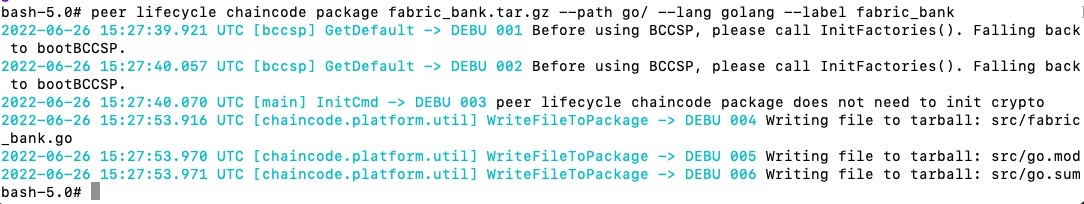
\includegraphics[width=0.7\textwidth]{./figs/archive.jpg}
        \caption{链码打包的结果截图}
    \end{figure}
    \begin{figure}[H]
        \centering
        \subfigure[中间命令的结果截图]{
            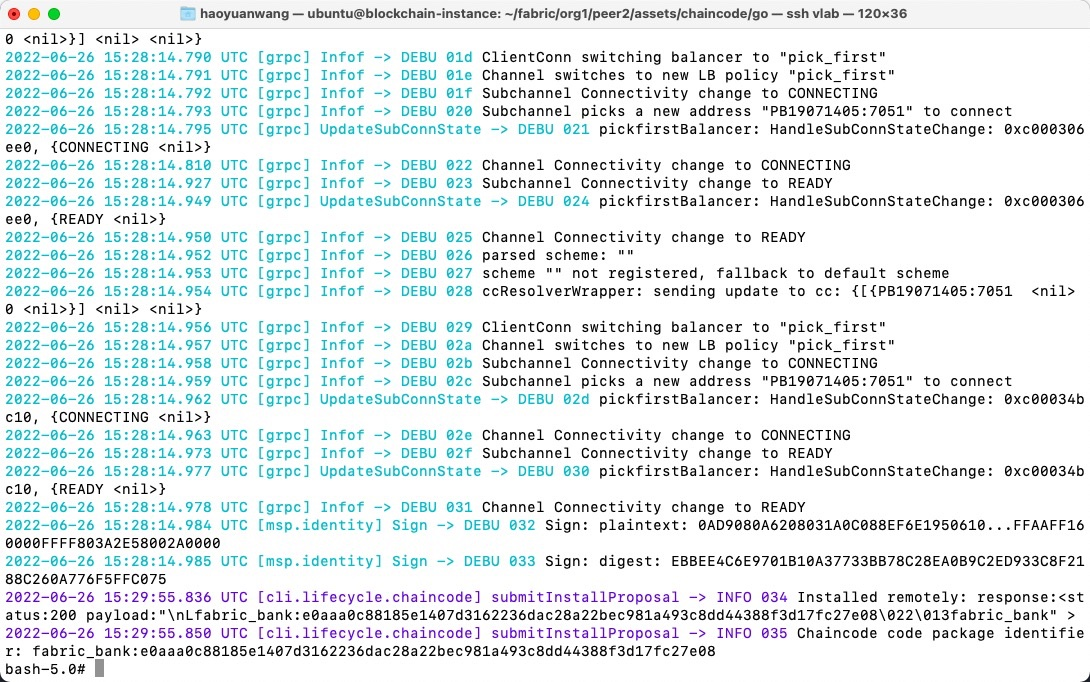
\includegraphics[width=0.4\textwidth]{./figs/install1.jpg}
        }
        \subfigure[最后命令的结果截图]{
            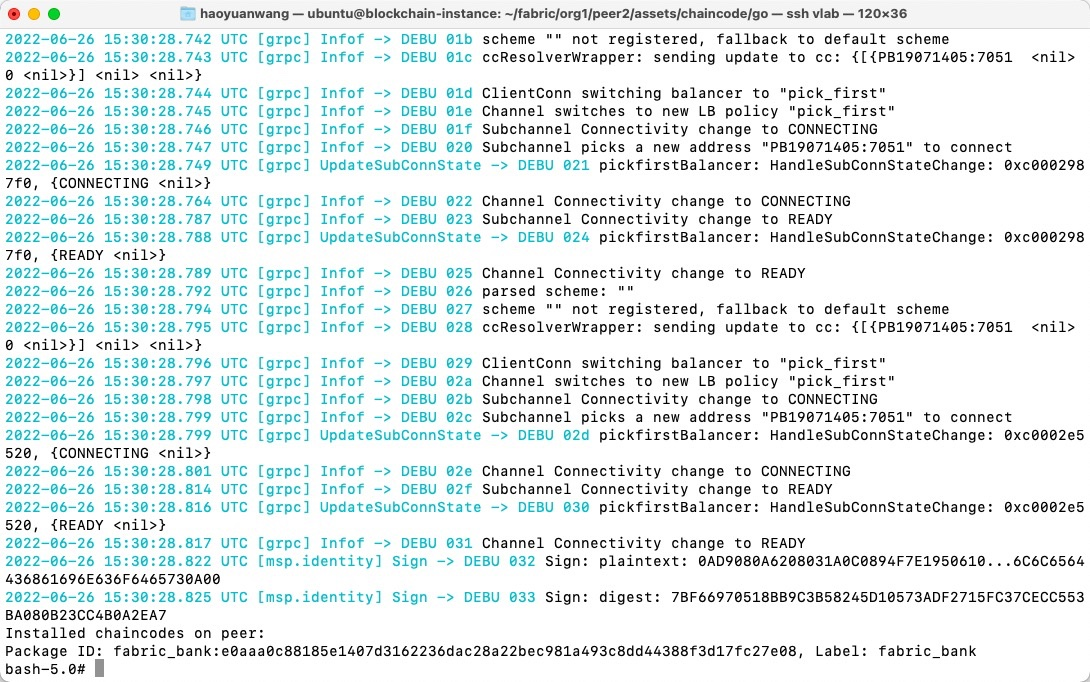
\includegraphics[width=0.4\textwidth]{./figs/install2.jpg}
        }
        \caption{链码安装的结果截图}
    \end{figure}
    \begin{figure}[H]
        \centering
        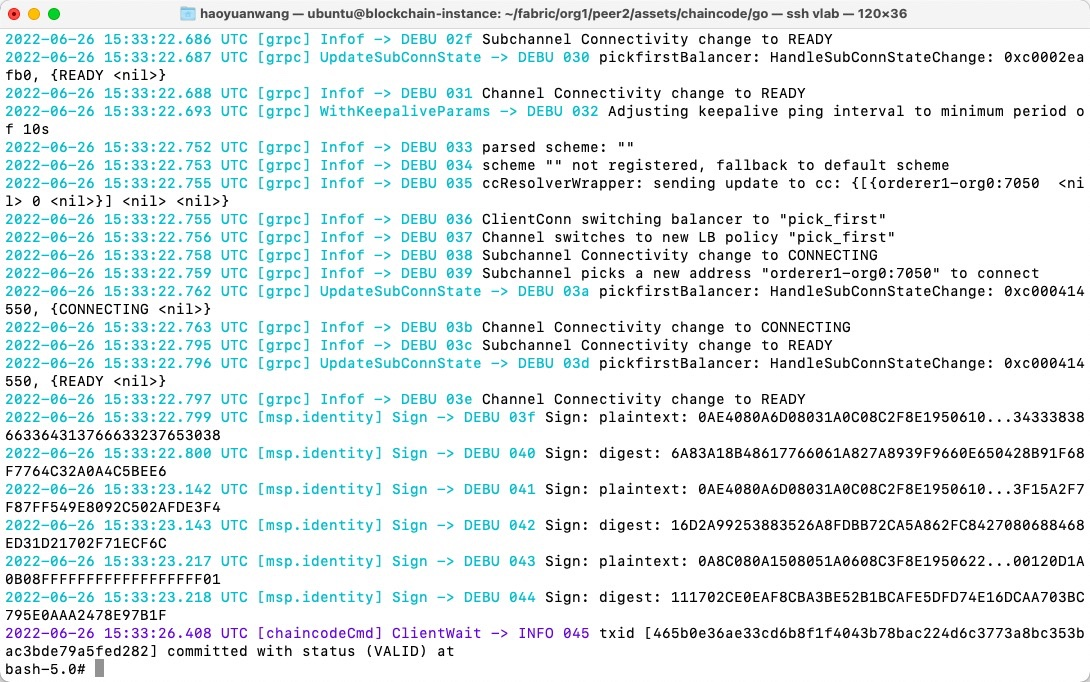
\includegraphics[width=0.7\textwidth]{./figs/准入.jpg}
        \caption{链码准入的结果截图}
    \end{figure}
    \begin{figure}[H]
        \centering
        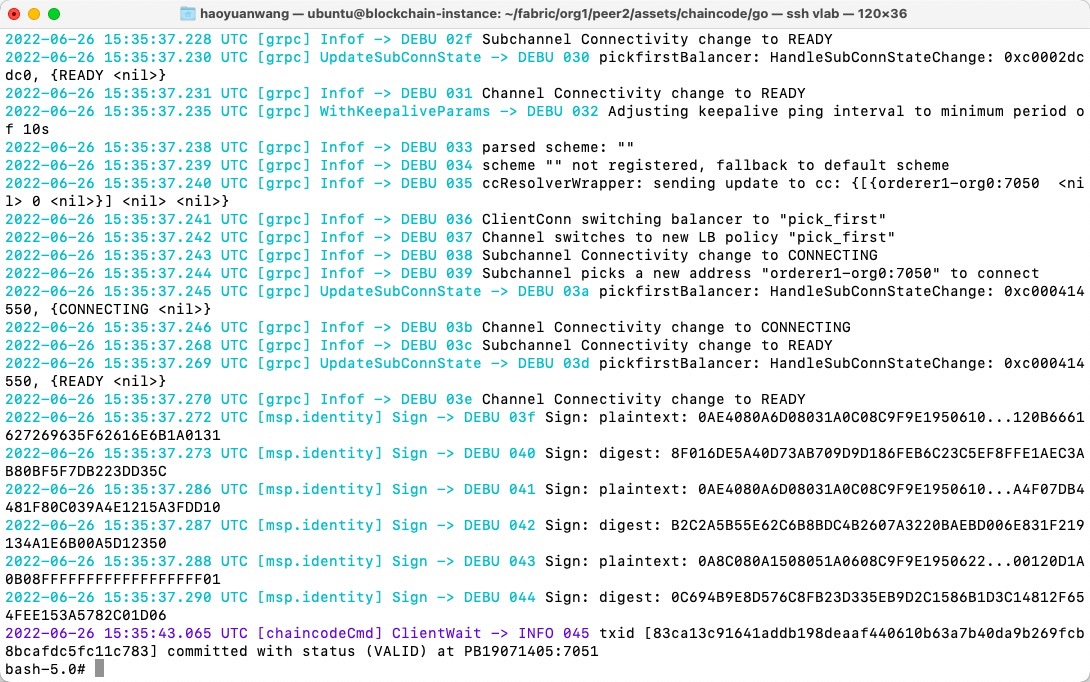
\includegraphics[width=0.7\textwidth]{./figs/上链.jpg}
        \caption{链码上链的结果截图}
    \end{figure}
    \begin{figure}[H]
        \centering
        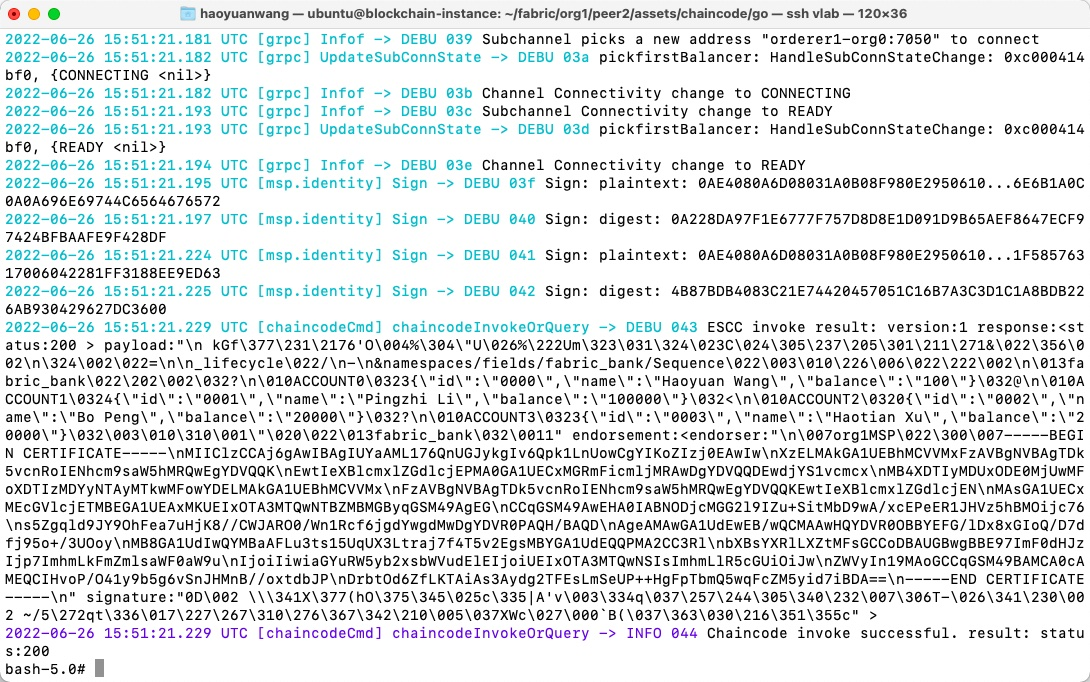
\includegraphics[width=0.7\textwidth]{./figs/init_result.jpg}
        \caption{初始化的结果截图}
    \end{figure}
    \begin{figure}[H]
        \centering
        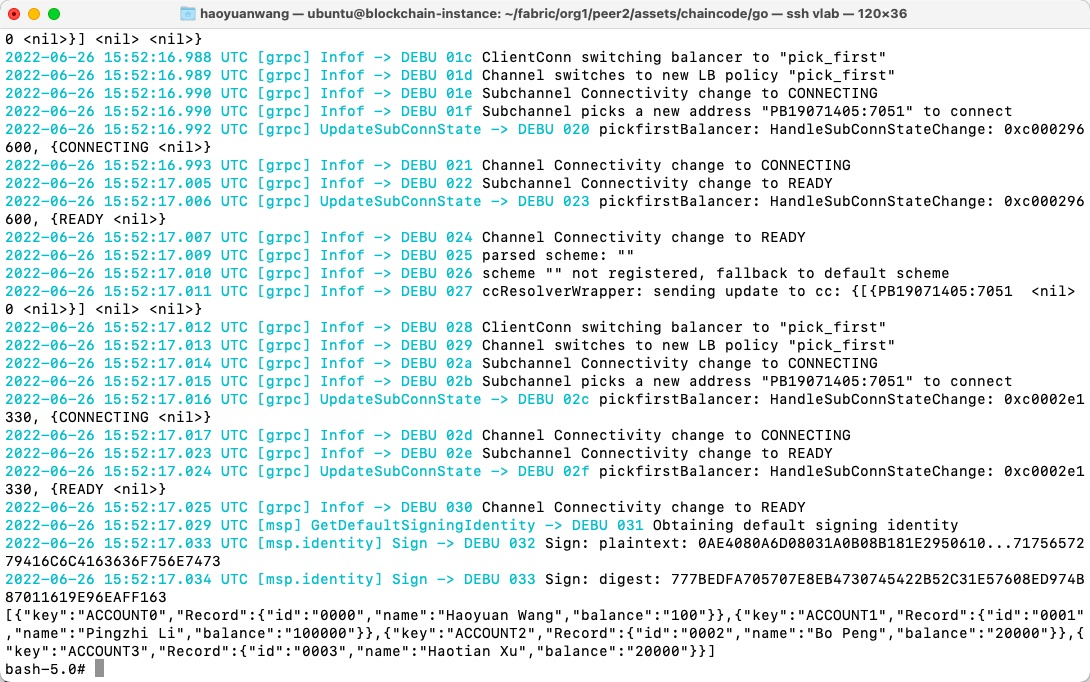
\includegraphics[width=0.7\textwidth]{./figs/invoke_result.jpg}
        \caption{请求所有账户的结果截图}
    \end{figure}
    \section{实验总结}
    由于考试和个人安排的缘故,导致实验时间紧张,有很多地方可能理解不是很透彻。
    但尽管如此,做完实验仍感觉到收获了很多,对超级账本的理解也更加深刻。
    对于区块链世界的应用和原理也产生了更多的兴趣。虽然这次实验完成的很仓促,
    有很多地方还很简陋(比如最开始其实想涉及更多的信息管理),但我学到了很多,
    也更加熟悉Fabric链码的相关操作。
\end{document}